\documentclass[a4paper,twoside]{article}
\usepackage[T1]{fontenc}
\usepackage[bahasa]{babel}
\usepackage{graphicx}
\usepackage{graphics}
\usepackage{float}
\usepackage[cm]{fullpage}
\pagestyle{myheadings}
\usepackage{etoolbox}
\usepackage{setspace} 
\usepackage{lipsum} 
\usepackage{amsmath}
\setlength{\headsep}{30pt}
\usepackage[inner=2cm,outer=2.5cm,top=2.5cm,bottom=2cm]{geometry} %margin
% \pagestyle{empty}

\makeatletter
\renewcommand{\@maketitle} {\begin{center} {\LARGE \textbf{ \textsc{\@title}} \par} \bigskip {\large \textbf{\textsc{\@author}} }\end{center} }
\renewcommand{\thispagestyle}[1]{}
\markright{\textbf{\textsc{Laporan Perkembangan Pengerjaan Skripsi\textemdash Sem. Ganjil 2019/2020}}}

\onehalfspacing
 
\begin{document}

\title{\@judultopik}
\author{\nama \textendash \@npm} 

%ISILAH DATA BERIKUT INI:
\newcommand{\nama}{Chris Eldon}
\newcommand{\@npm}{2016730073}
\newcommand{\tanggal}{25/11/2019} %Tanggal pembuatan dokumen
\newcommand{\@judultopik}{Privacy Preserving Data Mining dengan Metode Randomization} % Judul/topik anda
\newcommand{\kodetopik}{MTA4703}
\newcommand{\jumpemb}{1} % Jumlah pembimbing, 1 atau 2
\newcommand{\pembA}{Mariskha Tri Adithia, P.D.Eng}
\newcommand{\pembB}{-}
\newcommand{\semesterPertama}{47 - Ganjil 19/20} % semester pertama kali topik diambil, angka 1 dimulai dari sem Ganjil 96/97
\newcommand{\lamaSkripsi}{1} % Jumlah semester untuk mengerjakan skripsi s.d. dokumen ini dibuat
\newcommand{\kulPertama}{Skripsi 1} % Kuliah dimana topik ini diambil pertama kali
\newcommand{\tipePR}{B} % tipe progress report :
% A : dokumen pendukung untuk pengambilan ke-2 di Skripsi 1
% B : dokumen untuk reviewer pada presentasi dan review Skripsi 1
% C : dokumen pendukung untuk pengambilan ke-2 di Skripsi 2

% Dokumen hasil template ini harus dicetak bolak-balik !!!!

\maketitle

\pagenumbering{arabic}

\section{Data Skripsi} %TIDAK PERLU MENGUBAH BAGIAN INI !!!
Pembimbing utama/tunggal: {\bf \pembA}\\
Pembimbing pendamping: {\bf \pembB}\\
Kode Topik : {\bf \kodetopik}\\
Topik ini sudah dikerjakan selama : {\bf \lamaSkripsi} semester\\
Pengambilan pertama kali topik ini pada : Semester {\bf \semesterPertama} \\
Pengambilan pertama kali topik ini di kuliah : {\bf \kulPertama} \\
Tipe Laporan : {\bf \tipePR} -
\ifdefstring{\tipePR}{A}{
			Dokumen pendukung untuk {\BF pengambilan ke-2 di Skripsi 1} }
		{
		\ifdefstring{\tipePR}{B} {
				Dokumen untuk reviewer pada presentasi dan {\bf review Skripsi 1}}
			{	Dokumen pendukung untuk {\bf pengambilan ke-2 di Skripsi 2}}
		}
		
\section{Latar Belakang}
Dengan semakin banyaknya penambangan data yang dilakukan dan data yang digunakan juga semakin banyak, semakin banyak juga privasi di dalam data tersebut yang tersebar kepada pihak yang melakukan penambangan data. Data privasi tersebut dapat tersebar kepada pihak yang tidak bertanggung jawab dan disalahgunakan. Oleh karena itu perlu adanya suatu cara untuk mencegah privasi tersebar pada proses penambangan data, menjaga privasi pada data tersebut. Istilah untuk hal tersebut adalah \textit{privacy preserving data mining}.

Ada kesulitan dalam menentukan data seperti apa yang dapat disebut sebagai privasi. Privasi dapat dikatakan adalah sebuah informasi personal seseorang yang dapat mengidentifikasi suatu hal pada orang tersebut. Konsep yang sering kali digunakan untuk mendeskripsikan informasi personal adalah\textit{Personally Identifiable Information} yang disingkat PII. PII adalah segala informasi mengenai individu yang dikelola oleh sebuah instansi, termasuk segala informasi yang dapat digunakan untuk membedakan atau mengusut identitas seseorang dan juga segala informasi yang berhubungan atau dapat dihubungkan kepada suatu individu, seperti informasi medis, pendidikan, finansial, dan pekerjaan seseorang. 

Salah satu cara untuk melakukan \textit{privacy preserving data mining} adalah dengan melakukan modifikasi data yang ada sebelum diberikan kepada pihak lain. Ada macam-macam teknik dan algoritma yang bertujuan modifikasi data untuk \textit{privacy preserving data mining}, dibagi menjadi dua jenis yaitu \textit{Perturbation Approach} dan \textit{Anonymization Approach}. \textit{Perturbation Approach} adalah pendekatan untuk \textit{privacy preserving data mining} dengan cara mengacaukan data yang ada, tetapi hasil data yang dikacaukan masih tetap dapat ditambang. \textit{Perturbation Approach} dapat dibagi menjadi dua jenis yaitu \textit{Value-based Perturbation Techniques} dan \textit{Multi-Dimensional Perturbation}.

\textit{Value-based Perturbation Techniques} adalah teknik yang bekerja dengan cara menyisipkan \textit{random noise} pada data. Sedangkan terdapat dua jenis teknik \textit{Multi-Dimensional Perturbation} yaitu \textit{Data mining Task-based Perturbation} dan \textit{Dimension Reduction-based Perturbation}. \textit{Data mining Task-based Perturbation} adalah teknik yang bekerja dengan cara modifikasi data sehingga properti yang bertahan pada data yang telah dimodifikasi spesifik hanya properti yang digunakan oleh suatu teknik penambangan data tertentu. Sedangkan \textit{Dimension Reduction-based Perturbation} adalah teknik yang bekerja dengan cara modifikasi data sekaligus mengurangi dimensi dari data asli.

\begin{figure}
	\centering
	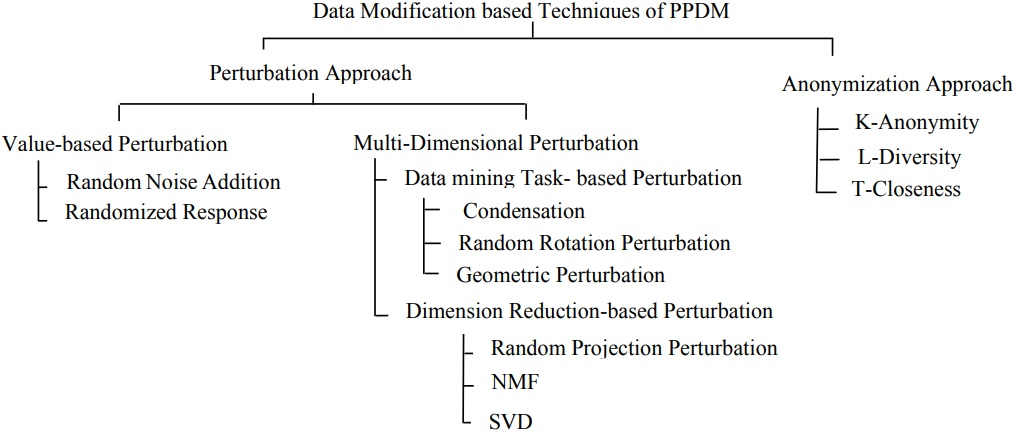
\includegraphics[scale=0.56]{ppdm}
	\caption{Berbagai macam teknik modifikasi data untuk \textit{privacy preserving data mining}}
	\label{fig:ppdm}
\end{figure}

Dari berbagai macam teknik modifikasi data untuk \textit{privacy preserving data mining} yang dapat dilihat pada Gambar~\ref{fig:ppdm}, terdapat empat teknik yang menggunakan metode \textit{Randomization} yaitu \textit{Random Noise Addition}, \textit{Randomized Response}, \textit{Random Rotation Perturbation}, dan \textit{Random Projection Perturbation}.

Pada penelitian ini, akan dibuat sebuah perangkat lunak yang dapat memproses data yang akan ditambang menjadi data yang telah dimodifikasi dengan metode \textit{Randomization} sehingga privasi pada data tersebut terlindungi, tetapi masih dapat ditambang. Dari berbagai macam teknik dengan metode \textit{Randomization} yang ada, dipilih dua buah teknik yaitu \textit{Random Rotation Perturbation} dan \textit{Random Projection Perturbation} untuk diimplementasikan pada perangkat lunak serta membandingkan hasil dari kedua teknik tersebut.

\section{Rumusan Masalah}
Berdasarkan latar belakang, rumusan masalah pada penelitian ini adalah sebagai berikut.
\begin{enumerate}
	\item Bagaimana cara kerja teknik \textit{Random Rotation Perturbation} dan \textit{Random Projection Perturbation} untuk \textit{privacy preserving data mining}?
	\item Bagaimana implementasi dari teknik \textit{Random Rotation Perturbation} dan \textit{Random Projection Perturbation} pada perangkat lunak?
	\item Bagaimana perbandingan antara hasil dari teknik \textit{Random Rotation Perturbation} dan \textit{Random Projection Perturbation}?
\end{enumerate}

\section{Tujuan}
Berdasarkan rumusan masalah, maka tujuan dari penelitian ini adalah sebagai berikut.
\begin{enumerate}
	\item Mempelajari cara kerja dari teknik \textit{Random Rotation Perturbation} dan \textit{Random Projection Perturbation} untuk \textit{privacy preserving data mining}
	\item Mengimplementasikan teknik \textit{Random Rotation Perturbation} dan \textit{Random Projection Perturbation} pada perangkat lunak
	\item Melakukan analisis dan pengujian untuk membandingkan dan mengukur hasil dari teknik \textit{Random Rotation Perturbation} dan \textit{Random Projection Perturbation}
\end{enumerate}

\section{Detail Perkembangan Pengerjaan Skripsi}
Detail bagian pekerjaan skripsi sesuai dengan rencana kerja/laporan perkembangan terakhir:
	\begin{enumerate}
		\item \textbf{Melakukan studi literatur mengenai dasar-dasar privasi data}\\
		{\bf Status :} Ada sejak rencana kerja skripsi.\\
		{\bf Hasil :} Pada umumnya sebuah data dapat dikatakan privasi apabila data tersebut dapat dikaitkan dengan identitas seseorang. Tetapi setiap orang memiliki kepentingan privasi yang berbeda-beda sehingga definisi dari privasi sulit untuk dijelaskan secara eksak. Oleh karena itu, perlu adanya konsep privasi yang dapat menjadi acuan untuk menentukan data seperti apa yang termasuk privasi atau bukan.
		\begin{enumerate}
			\item Privasi
			
			Dalam mendefinisikan privasi, sulit untuk mendapatkan definisi yang tepat untuk privasi karena setiap individu memiliki kepentingan yang berbeda-beda sehingga privasi pada setiap individu dapat berbeda-beda juga. Beberapa definisi privasi telah dikemukakan dan definisi tersebut bermacam-macam berdasarkan konteks, budaya, dan lingkungan. Menurut Warren dan Brandeis pada papernya, mereka mendefinisikan privasi sebagai “\textit{the right to be alone.}”, hak untuk menyendiri. Lalu pada papernya, Westin mendefinisikan privasi sebagai “\textit{the desire of people to choose freely under what circumstances and to what extent they will expose themselves, their attitude, and their behavior to others}”, keinginan orang untuk memilih secara bebas dalam segala situasi dan dalam hal mengemukakan diri mereka, sikap mereka, dan tingkah laku mereka pada orang lain. 
			
			Schoeman mendefinisikan privasi sebagai “\textit{the right to determine what (personal) information is communicated to others}”, hak untuk menentukan informasi pribadi apa saja yang dikomunikasikan kepada yang lain, atau “\textit{the control an individual has over information about himself or herself.}”, kendali seorang individu terhadap informasi tentang dirinya sendiri. Lalu baru-baru ini, Garfinkel menyatakan bahwa “\textit{privacy is about self-possession, autonomy, and integrity.}”, privasi adalah tentang penguasaan diri sendiri, otonomi, dan integritas. Di samping itu, Rosenberg berpendapat bahwa privasi sebenarnya bukan sebuah hak tetapi sebuah rasa: “\textit{If privacy is in the end a matter of individual taste, then seeking a moral foundation for it -- beyond its role in making social institutions possible that we happen to prize -- will be no more fruitful than seeking a moral foundation for the taste for truffles.}”, intinya setiap orang memiliki perhatian yang berbeda-beda terhadap privasi mereka sendiri sehingga hal tersebut tergantung apa yang dirasakan oleh setiap individu.

			Dari definisi-definisi privasi yang telah disebutkan di atas, dapat disimpulkan bahwa privasi dilihat sebagai konsep sosial dan budaya. Konsep privasi pada suatu lingkungan dapat berbeda dari lingkungan lainnya dan hal ini menyebabkan sulitnya menentukan apakah sebuah data termasuk privasi atau bukan. Oleh karena itu, perlu adanya sebuah standar privasi untuk menentukan data mana yang dapat disebut sebuah privasi. Organisasi National Institute of Standards and Technology dari Amerika Serikat, membuat standar mereka sendiri untuk menentukan informasi seperti apa yang dapat disebut sebagai privasi. Mereka mengemukakan konsep \textit{Personally Identifiable Information} sebagai informasi yang dapat dikatakan personal untuk setiap individu.

			\item \textit{Personally Identifiable Information}
			
			Privasi dapat dikatakan adalah sebuah informasi personal seseorang yang dapat mengidentifikasi suatu hal pada orang tersebut. Konsep yang sering kali digunakan untuk mendeskripsikan informasi personal adalah \textit{Personally Identifiable Information} yang disingkat PII. PII adalah segala informasi mengenai individu yang dikelola oleh sebuah instansi, termasuk segala informasi yang dapat digunakan untuk membedakan atau mengusut identitas seseorang dan juga segala informasi yang berhubungan atau dapat dihubungkan kepada suatu individu, seperti informasi medis, pendidikan, finansial, dan pekerjaan seseorang. 

			Informasi yang termasuk membedakan individu adalah informasi yang dapat mengidentifikasi seorang individu. Informasi seperti ini adalah data privasi yang secara langsung bisa didapatkan. Beberapa contoh informasi yang mengidentifikasi seorang individu adalah nama, nomor KTP, tempat tanggal lahir, nama ibu kandung, atau catatan medis. Sedangkan, data yang hanya berisi misalkan saldo tabungan tanpa ada informasi lain mengenai identitas seseorang yang berkaitan tidak menyediakan informasi yang cukup untuk mengidentifikasi seorang individu.

			Dari sebuah data, bisa saja data tersebut secara tidak langsung mengandung privasi, identitas seseorang bisa didapatkan tanpa data tersebut memberikan langsung identitas orang tersebut. Mengusut identitas seseorang adalah proses dari membuat perkiraan tentang aspek spesifik dari aktivitas atau status seseorang. Jika sebuah data dapat dianalisis datanya sampai identitas seseorang dapat diakses, berarti data tersebut secara tidak langsung mengandung privasi. Contohnya adalah sebuah catatan finansial seseorang dapat digunakan untuk memperkirakan aktivitas dari individu tersebut.

			Informasi yang berhubungan dapat didefinisikan sebagai informasi yang berkaitan dengan seorang individu yang mana terkait secara logis dengan informasi lain tentang individu tersebut. Informasi tersebut secara tidak langsung mengandung privasi dan dapat diolah agar identitas seseorang bisa didapatkan. Contohnya adalah apabila ada dua buah basis data yang memiliki data berbeda dari seorang individu, maka seseorang yang memiliki akses pada 2 basis data tersebut berpotensi dapat mengaitkan data-data tersebut lalu mengidentifikasi individu yang ada pada data tersebut.
		\end{enumerate}

		\item \textbf{Melakukan studi literatur mengenai penambangan data dan tekniknya}\\
		{\bf Status :} Ada sejak rencana kerja skripsi.\\
		{\bf Hasil :} Pada era teknologi informasi, sangat banyak data terkumpul pada basis data. Data yang masif ini dapat dimanfaatkan untuk menggali informasi penting yang berguna untuk pembuatan keputusan. Proses pada aktivitas ini secara kasar dapat disebut dengan penambangan data.

		Penambangan data adalah proses mengekstrak sebuah pola atau sebuah pengetahuan dari kumpulan data yang besar, yang mana dapat direpresentasikan dan diinterpretasikan. Pada penambangan data, teknik \textit{machine learning} dan \textit{pattern recognition} intensif digunakan untuk mendapatkan pola maupun pengetahuan baru dari data. Tujuan utama dari penambangan data adalah untuk membentuk model deskriptif dan prediktif dari suatu data. Model deskriptif berusaha untuk mengubah pola-pola yang ada pada data menjadi deskripsi yang dapat dimengerti oleh orang awam. Sedangkan model prediktif digunakan untuk memprediksi data yang tidak diketahui atau data yang berpotensi muncul di kemudian hari.
		
		Model tersebut biasanya dibuat dengan menggunakan teknik \textit{machine learning}, yang mana terdapat dua teknik \textit{machine learning} yang paling sering digunakan yaitu \textit{classification} dan \textit{clustering}. Subbab berikutnya akan menjelaskan secara singkat kedua teknik tersebut dan contoh algoritmanya.

		\begin{enumerate}
			\item \textit{Classification}
			
			Tujuan utama \textit{Classification} (klasifikasi) adalah membuat model yang dalam kasus ini disebut \textit{classifier} yang mana dapat mengidentifikasi nilai kelas dari suatu data. Dalam kata lain, sebuah \textit{classifier} dibuat dari sebuah \textit{training set} dan model ini digunakan untuk mengklasifikasi data tidak diketahui ke dalam salah satu kelas. Ada dua tahap dalam proses klasifikasi yaitu tahap latihan dan tahap klasifikasi.

			Pada tahap latihan, model akan dibuat dengan menggunakan \textit{training set}. \textit{Training set} yang dimaksud adalah data yang sudah diketahui kelasnya sehingga model yang ada melatih dirinya. Setelah \textit{classifier} terbentuk, barulah tahap klasifikasi dapat dilakukan dengan menggunakan \textit{classifier} yang tadi sudah dibuat. \textit{Classifier} akan memprediksi data yang kelasnya tidak diketahui. \textit{Classifier} akan semakin baik performanya seiring dengan banyaknya tahap latihan yang dilakukan.

			Teknik \textit{machine learning} yang paling dikenal untuk klasifikasi antara lain \textit{K-nearest Neighbors}, \textit{Decision Tree}, dan \textit{Naive Bayes}. Dalam penelitian ini, hanya teknik \textit{K-nearest Neighbors} yang digunakan untuk pengujian sehingga berikutnya hanya akan dijelaskan teknik \textit{K-nearest Neighbors} saja.

			Teknik \textit{K-nearest Neighbors} adalah teknik penambangan data klasifikasi yang mencari label terbanyak pada sejumlah tetangga terdekatnya. Teknik ini bergantung pada jarak Euclidean antara titik yang mana adalah data yang akan diprediksi dengan tetangga-tetangganya. Setiap rekord pada data dipetakan ke bidang Euclidean dengan beberapa atribut yang menentukan letaknya pada bidang Euclidean. 

			Berikut langkah kerja dari teknik \textit{K-nearest Neighbors}.
			\begin{enumerate}
				\item Tentukan nilai \(k\) yang menentukan seberapa banyak tetangga yang digunakan
				\item Lakukan perulangan dengan iterasi sebanyak rekord yang ada selain rekord yang ingin diprediksi labelnya
				\begin{enumerate}
					\item Hitung jarak Euclidean antara rekord iterasi sekarang dengan rekord yang ingin diprediksi labelnya
					\item Catat jarak Euclidean dari rekord yang ingin diprediksi dan indeks rekord iterasi sekarang
				\end{enumerate}
				\item Urutkan jarak Euclidean titik-titik yang sudah dihitung pada perulangan pada langkah sebelumnya secara menaik
				\item Pilih rekord teratas (jarak Euclidean yang paling kecil) sebanyak \(k\) dari urutan pada langkah sebelumnya
				\item Ambil label dari semua rekord yang terpilih pada langkah sebelumnya. Label terbanyak adalah hasil prediksi label pada rekord yang ingin diprediksi
			\end{enumerate}
			
			\item \textit{Clustering}
			
			\textit{Clustering} adalah proses mengelompokan kumpulan objek ke dalam sebuah kelompok (\textit{cluster}) sedemikian rupa sehingga objek-objek dari suatu \textit{cluster} memiliki lebih banyak kemiripan dari pada objek-objek dari \textit{cluster} lainnya. 

			Salah satu contoh teknik \textit{clustering} adalah \textit{K-means}. Teknik \textit{k-means} adalah adalah teknik penambangan data \textit{clustering} yang memanfaatkan jarak Euclidean antara titik-titik yang ada untuk menentukan titik mana saja yang masuk ke kluster mana.

			Berikut langkah kerja dari teknik \textit{K-means}.
			\begin{enumerate}
				\item Tentukan nilai \(k\) yang menentukan seberapa banyak kluster yang diinginkan dan sebuah \textit{treshold} untuk menentukan batas perubahan nilai centroid
				\item Tentukan secara acak sebuah centroid sebanyak \(k\)  untuk setiap kluster
				\item Lakukan perulangan sampai nilai fitur-fitur semua centroid (titik tengah kluster) relatif tidak berubah atau dengan kata lain perubahannya kurang dari \textit{treshold}
				\begin{enumerate}
					\item Menghitung jarak Euclidean tiap titik dari centroid ke titik tersebut dengan menggunakan beberapa fitur yang dipilih
					\item Kluster yang memiliki jarak Euclidean paling kecil dengan sebuah titik adalah kluster titik tersebut
					\item Tentukan kembali centroid setiap kluster dengan cara menghitung rata-rata tiap fitur seluruh data pada kluster tersebut
				\end{enumerate}
			\end{enumerate}
		\end{enumerate}

		\item \textbf{Melakukan studi literatur mengenai \textit{privacy preserving data mining}}\\
		{\bf Status :} Ada sejak rencana kerja skripsi.\\
		{\bf Hasil :} Aktivitas penambangan data melibatkan jumlah data yang sangat masif. Data-data yang digunakan memiliki privasi banyak individu di dalamnya. Hal ini berpotensi menyebabkan pelanggaran privasi dalam kasus tidak adanya proteksi yang cukup dan penyalahgunaan privasi data untuk tujuan lain. Faktor utama pelanggaran privasi pada penambangan data adalah penyalahgunaan data sehingga hal ini dapat merugikan seorang individu maupun sebuah organisasi. Oleh karena itu, ada kebutuhan untuk menghindari penyebaran informasi pribadi yang rahasia maupun pengetahuan lainnya yang dapat diambil dari data yang digunakan untuk aktivitas penambangan data.
		
		Konsep privasi sering kali lebih kompleks dari pada yang dibayangkan. Dalam kasus penambangan data, definisi dari menjaga privasi masih tidak jelas. Ada sebuah paper yang mendefinisikan \textit{privacy preserving data mining} sebagai “getting valid data mining results without learning the underlying data values”, mendapatkan hasil penambangan data yang valid tanpa  nilai pada data. Tetapi pada saat ini setiap teknik \textit{privacy preserving data mining} yang ada memiliki definisi privasinya masing-masing. 
		
		Salah satu cara untuk melakukan \textit{privacy preserving data mining} adalah dengan melakukan modifikasi data yang ada sebelum diberikan kepada pihak lain. Berbagai macam pendekatan modifikasi data untuk \textit{privacy preserving data mining} telah dikembangkan antara lain \textit{Perturbation Approach} dan \textit{Anonymization Approach}, selengkapnya dapat dilihat pada Gambar~\ref{fig:ppdm}. \textit{Perturbation Approach} adalah pendekatan untuk \textit{privacy preserving data mining} dengan cara mengacaukan data yang ada, tetapi hasil data yang dikacaukan masih tetap dapat ditambang. Sedangkan pada \textit{Anonymization Approach}, data diterapkan de-identifikasi di mana \textit{dataset} mentah disebarluaskan setelah menghapus inti dari identitas setiap rekord.
		
		\textit{Perturbation Approach} dapat dibagi menjadi dua jenis lagi yaitu \textit{Value-based Perturbation Techniques} dan \textit{Multi-Dimensional Perturbation}. \textit{Value-based Perturbation Techniques} adalah teknik yang bekerja dengan cara menyisipkan \textit{random noise} pada data. Sedangkan terdapat dua jenis teknik \textit{Multi-Dimensional Perturbation} yaitu \textit{Data mining Task-based Perturbation} dan \textit{Dimension Reduction-based Perturbation}. \textit{Data mining Task-based Perturbation} adalah teknik yang bekerja dengan cara modifikasi data sehingga properti yang bertahan pada data yang telah dimodifikasi spesifik hanya properti yang digunakan oleh suatu teknik penambangan data tertentu. Sedangkan \textit{Dimension Reduction-based Perturbation} adalah teknik yang bekerja dengan cara modifikasi data sekaligus mengurangi dimensi dari data asli.
		
		Hal yang sering kali diperhatikan pada teknik-teknik \textit{Perturbation Approach} adalah perbandingan antara jumlah privasi yang hilang dan jumlah informasi yang hilang. Idealnya teknik \textit{Perturbation Approach} yang baik adalah teknik yang fokus meminimalkan jumlah privasi yang hilang dan jumlah informasi yang hilang sehingga hasil penambangan dan akurasinya sama baiknya dengan tanpa menerapkan teknik \textit{Perturbation Approach}. Setiap teknik penambangan data memakai properti yang berbeda-beda pada data yang ditambang. Oleh karena itu, properti yang terjaga pun sebaiknya berdasarkan properti yang digunakan pada teknik penambangan data yang digunakan. Pada saat ini, teknik modifikasi data yang ada sering kali memiliki perbedaan pada properti-properti yang terjaga. Teknik-teknik modifikasi data tertentu sering kali memiliki fungsi yang berbeda atau teknik penambangan data yang dapat digunakan berbeda karena properti yang terjaga pada teknik-teknik tersebut berbeda juga.

		\item \textbf{Melakukan studi literatur mengenai metode \textit{Randomization}}\\
		{\bf Status :} Ada sejak rencana kerja skripsi.\\
		{\bf Hasil :} Dari berbagai macam teknik modifikasi data untuk \textit{privacy preserving data mining} yang dapat dilihat pada Gambar~\ref{fig:ppdm}, terdapat empat teknik yang menggunakan metode \textit{Randomization} yaitu \textit{Random Noise Addition}, \textit{Randomized Response}, \textit{Random Rotation Perturbation}, dan \textit{Random Projection Perturbation}.

		Berbagai macam teknik dengan metode randomisasi umumnya menerapkan perusakan nilai pada data. Salah satu teknik yang pertama kali menggunakan metode randomisasi untuk \textit{privacy preserving data mining} adalah teknik \textit{Random Noise Addition} yang dikemukakan oleh Agrawal dan Srikant pada paper berikut. Teknik \textit{Random Noise Addition} ini dilakukan dengan cara menambahkan nilai random (\textit{noise}) pada data. Nilai random tersebut diambil dari sebuah distribusi. Untuk menambang data yang telah ditambahkan \textit{noise} ini perlu dilakukan rekonstruksi distribusi untuk mendapatkan distribusi yang asli. Oleh karena itu, teknik \textit{Random Noise Addition} ini hanya menjaga distribusi data asli sehingga hanya teknik penambangan data yang bergantung pada distribusi data saja yang dapat digunakan. Penyesuaian pada algoritma penambangan data yang digunakan pun perlu dilakukan agar teknik \textit{Random Noise Addition} ini dapat digunakan dan mendapatkan hasil penambangan data yang hampir sama dengan tanpa menggunakan teknik \textit{Random Noise Addition}.
		
		Setelah teknik \textit{Random Noise Addition} ditemukan, berbagai macam teknik lain pun dikembangkan terinspirasi dari teknik \textit{Random Noise Addition} ini. Teknik \textit{Random Rotation Perturbation} dan \textit{Random Projection Perturbation} adalah teknik adalah salah satunya, tetapi teknik tersebut tidak dilakukan dengan cara menambahkan \textit{noise} melainkan mengkalikan data asli dengan nilai random. Bagaimanapun juga, inti dari teknik-teknik \textit{Randomization} yang telah disebutkan di atas masih sama yaitu merusak data sehingga data yang dirilis bukanlah data asli melainkan data yang sudah rusak sehingga data yang dirilis tidak mengandung privasi dan privasi pun terjaga.
		
		\item \textbf{Melakukan studi literatur dan mempelajari teknik \textit{Random Noise Addition}}\\
		{\bf Status :} Ada sejak rencana kerja skripsi tetapi tidak dilanjutkan.\\
		{\bf Hasil :} Ide utama dari teknik \textit{Random Noise Addition} adalah mendistorsi nilai pada data dengan cara menambahkan \textit{random noise} yang diambil dari distribusi \textit{Uniform} atau \textit{Gaussian} dan memiliki rata-rata bernilai 0. Tetapi menurut penelitian yang telah dilakukan, distribusi \textit{Gaussian} lebih baik digunakan untuk teknik ini. \textit{Random noise} yang digunakan memiliki nilai yang berbeda untuk setiap nilai pada data.

		Dengan teknik \textit{Random Noise Addition}, dari data yang sudah didistorsi bisa didapatkan kembali distribusi data asli dengan merekonstruksi distribusinya tanpa mendapatkan setiap nilai-nilai yang ada pada data asli. Metode rekonstruksi yang digunakan berdasarkan pada aturan \textit{Bayes}. Algoritma rekonstruksi untuk mendapatkan distribusi dari data asli dapat dilihat pada Gambar~\ref{fig:rnaalgorithm}.
		
		\begin{figure}
			\centering
			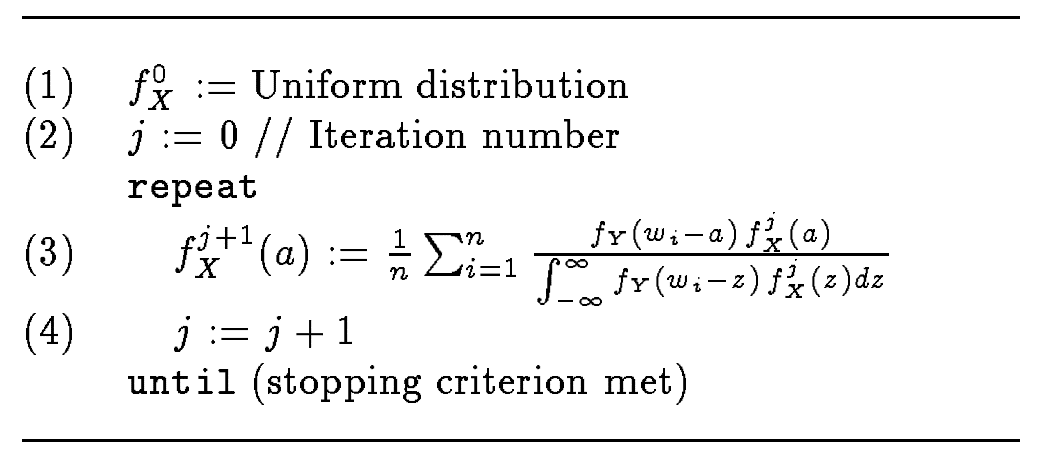
\includegraphics[scale=0.4]{rnaalgorithm}
			\caption{Algoritma rekonstruksi}
			\label{fig:rnaalgorithm}
		\end{figure}

		Algoritma ini berhenti sampai kriteria berhentinya terpenuhi. Kriteria tersebut adalah perbedaan estimasi distribusi iterasi sekarang dengan yang sebelumnya sangat kecil. Algoritma ini akan menghasilkan estimasi distribusi data asli dengan menggunakan data yang telah terdistorsi tanpa menggunakan nilai-nilai pada data asli, sehingga nilai-nilai pada data asli tidak tersebar. Oleh karena teknik \textit{Random Noise Addition} hanya menjaga distribusi pada data maka teknik penambangan data yang dapat digunakan hanya teknik-teknik yang bergantung pada distribusi data saja.

		Modifikasi pada algoritma penambangan data yang digunakan pun perlu dilakukan. Contohnya apabila algoritma pohon keputusan digunakan, maka perlu modifikasi pada algoritma pohon keputusan tersebut. Hal ini menimbulkan masalah pada aplikasi pada dunia nyata karena tidak efisien dan memakan waktu untuk memodifikasi setiap algoritma yang ingin digunakan untuk menyesuaikan dengan teknik \textit{Random Noise Addition}. Masalah mengenai algoritma yang dapat digunakan pun menjadi perhatian karena teknik \textit{Random Noise Addition} hanya dapat digunakan untuk algoritma yang bergantung pada distribusi saja sedangkan teknik \textit{Randomization} lain tidak menjaga distribusi pada data. Ada juga penelitian yang mengatakan bahwa teknik \textit{Random Noise Addition} ini memiliki kualitas yang kurang baik dalam menjaga privasi data karena banyaknya celah yang dapat diserang pada teknik ini. Oleh karena masalah-masalah tersebut, akhirnya teknik ini pun tidak akan digunakan untuk diuji kualitas hasilnya. Teknik \textit{Random Projection Perturbation} akan digunakan untuk menggantikan teknik \textit{Random Noise Addition}.

		\item \textbf{Melakukan studi literatur dan mempelajari teknik \textit{Random Rotation Perturbation}}\\
		{\bf Status :} Ada sejak rencana kerja skripsi.\\
		{\bf Hasil :} Ide utama dari teknik \textit{Random Rotation Perturbation} adalah jika data direpresentasikan sebagai matrix \(X_{n \times d}\) , \textit{rotation perturbation} dari \textit{dataset} X didefinisikan sebagai berikut.
		\begin{equation}
			G(X) = X_{n \times d} R_{d \times d}
		\end{equation}
		Dimana \(R_{d \times d}\) adalah \textit{random rotation matrix}. \textit{Random rotation matrix} berukuran \(d\) dimensi dapat dibuat dengan cara membuat matriks \textit{special orthogonal} acak karena matriks rotasi memiliki sifat {special orthogonal}. Matriks \textit{special orthogonal} adalah matriks yang memiliki sifat \textit{orthogonal} dan determinannya bernilai +1, yang mana matriks \textit{orthogonal} adalah matriks yang menghasilkan matriks identitas apabila dikalikan dengan transposenya sendiri. Matriks rotasi ini dapat dibuat secara efisien mengikuti distribusi Haar. Dari definisi di atas dapat disimpulkan tranformasi rotasi tersebut menjaga jarak Euclidean.
		
		Teknik ini menjaga beberapa properti pada data antara lain yaitu jarak Euclidean, \textit{inner product}, dan \textit{geometric shape hyper} pada bidang multi-dimensi. Oleh karena itu, beberapa teknik penambangan data tidak berpengaruh (dapat digunakan) terhadap teknik \textit{Random Rotation Perturbation} antara lain yaitu \textit{K-nearest Neighbors}, \textit{Support Vector Machines}, dan \textit{Perceptrons}. Teknik ini dipercaya dapat memberikan hasil penambangan yang maksimal, hasil penambangan data yang telah dirusak persis sama dengan hasil penambangan data aslinya. Sehingga jumlah informasi yang hilang tidak ada, tetapi jumlah privasi yang hilangnya tinggi. Walaupun demikian ada beberapa penelitian yang mengatakan bahwa karena teknik \textit{Random Rotation Perturbation} ini memiliki sifat demikian sehigga teknik ini dikatakan tidak aman dan dapat diserang dengan beberapa teknik untuk mendapatkan data asli yang lengkap.
		
		Transformasi translasi juga perlu dilakukan agar rotasi yang dilakukan merusak data secara menyeluruh. Apabila tidak dilakukan translasi, nilai pada data yang mendekati nilai nol akan menghasilkan nilai yang mendekati nol juga setelah dirotasi. Implikasi dari hal tersebut adalah lemahnya dalam menjaga privasi. Translasi dapat dilakukan dengan cara membuat matriks translasi yang acak lalu kalikan dengan matriks data asli. Translasi dapat dilakukan karena translasi tidak mengubah properti geometris dari matriks yang ditranslasi sehingga jarak Euclidean dan properti lainnya pun terjaga dan hasil penambangan data pun tetap sama.

		\item \textbf{Melakukan studi literatur dan mempelajari teknik \textit{Random Projection Perturbation}} \\
		{\bf Status :} Ditambahkan untuk menggantikan teknik \textit{Random Noise Addition}.\\
		{\bf Hasil :} Ide utama dari teknik \textit{Random Projection Perturbation} adalah mereduksi dimensi dari representasi matriks data asli dengan syarat dimensi matriks tersebut cukup besar. Dasar dari teknik \textit{Random Projection Perturbation} berdiri pada \textit{Johnson-Lindenstrauss Lemma}. 
		\newtheorem{theorem}{Lemma}
		\begin{theorem}[\textit{JOHNSON-LINDENSTRAUSS LEMMA}]
			For any \(0 < \epsilon < 1\) and any integer \(s\), let \(k\) be a positive integer such that \(k\) \(\geq 4(\epsilon^{2}/2-\epsilon^{3}/3)^{-1}\ln{n}\). Then, for any set \(S\) of \(s = |S|\) data points in \({\rm I\!R}^{m}\), there is a map \(f : {\rm I\!R}^{m} \rightarrow {\rm I\!R}^{k}\) such that, for all \(x, y \in S\), \((1-eps)||u - v||^{2}<||p(u) - p(v)||^{2}<(1+eps)||u - v||^{2}\), where \(||.||\) denotes the vector 2-norm.
		\end{theorem}
		Inti dari Lemma ini menunjukkan bahwa titik pada bidang Euclidean \(d\)-dimensi dapat diproyeksikan ke bidang Euclidean berdimensi lebih kecil dari \(d\), sedemikian rupa sehingga jarak antara dua titik tetap konsisten dengan \textit{error} yang terkontrol tetapi dengan syarat \(d\) harus cukup besar. Oleh karena adanya \textit{error} yang muncul, properti-properti pada data pun relatif sedikit berubah dan hal ini menyebabkan akurasi pada model yang dibuat dengan data tersebut berkurang dibandingkan data aslinya.
		
		\textit{Projection perturbation} dari \textit{dataset} X didefinisikan sebagai berikut.
		\begin{equation}
			G(X) = X_{n \times d} R_{d \times k}
		\end{equation}
		Dimana \(R_{d \times k}\) adalah \textit{random projection matrix} yang dihasilkan mengikuti distribusi normal, dengan rata-rata bernilai 0 dan standar deviasi bernilai \(1/\sqrt{k}\). Ukuran matriks \(R_{d \times k}\) disesuaikan dengan matriks \(X_{n \times d}\) yang mana \textit{dataset} asli dengan jumlah rekord \(n\) dan jumlah atribut \(d\), yang mana \(d\) akan menjadi dimensi matriks. Oleh karena yang ingin dilakukan adalah reduksi dimensi maka \(k\) harus lebih kecil dari pada \(d\), yang mana \(k\) adalah dimensi dari matriks baru yang dihasilkan dari \textit{Random Projection Perturbation} ini.
		
		Jika \textit{random projection matrix} yang digunakan dihasilkan secara acak saja, hasil dari \textit{random projection perturbation} akan terlalu merusak nilai pada data sehingga akurasi pada model yang akan dibuat kemungkinan berkurang drastis. Cara menanggulangi hal tersebut adalah menggunakan matriks \textit{orthogonal} sebagai \textit{random projection matrix}. Tetapi membuat matriks \textit{orthogonal} yang berdimensi tinggi memiliki kompleksitas yang tinggi sehingga memerlukan \textit{cost} yang besar. Pada observasi yang dilakukan Hecht-Neilsen menunjukkan bahwa “\textit{that in a high-dimensional space, vectors with random directions are almost orthogonal}”. Dapat disimpulkan bahwa dalam kasus matriks berdimensi tinggi apabila sebuah matriks dihasilkan secara acak mengikuti suatu distribusi, matriks tersebut akan kurang lebih hampir \textit{orthogonal}. Oleh karena itu, matriks yang dibuat untuk \textit{Random Projection Perturbation} cukup matriks acak yang mengikuti suatu distribusi saja.
		
		Menurut \textit{Johnson-Lindenstrauss Lemma}, reduksi dimensi pada matriks berdimensi tinggi minimal berdimensi \(k\), yang mana \(k\) didefinisikan sebagai berikut.
		\begin{equation}
			k \geq 4(\epsilon^{2}/2-\epsilon^{3}/3)^{-1}\ln{n}
		\end{equation}
		Sebuah matriks yang akan diproyeksikan ke dimensi yang lebih kecil akan memiliki nilai \textit{error} pada jarak Euclidean yang dimiliki oleh titik-titik (setiap elemen dari matriks) pada bidang Euclidean tersebut. Nilai \textit{error} tersebut ditentukan oleh variabel \(\epsilon\), yang mana \(\epsilon\) menjadi ukuran seberapa baik proyeksi dilakukan. Semakin kecil nilai \(\epsilon\) maka semakin besar \(k\), yang mana \(k\) adalah dimensi minimal matriks yang dihasilkan. Semakin titik-titik pada bidang Euclidean diproyeksikan ke dimensi lebih kecil, semakin besar kerusakan yang timbul pada jarak Euclidean titik-titik tersebut.
		
		Persamaan berikut menyatakan rentang error yang terjadi pada \textit{Random Projection Perturbation} dengan \(\epsilon\) (eps) yang ditentukan berada pada rentang (0, 1). 
		\begin{equation}
			(1-eps)||u - v||^{2}<||p(u) - p(v)||^{2}<(1+eps)||u - v||^{2}
		\end{equation}
		Pada hasil proyeksi, jarak Euclidean antara suatu titik dengan suatu titik lainnya dapat dipastikan berada pada rentang tersebut dan tidak akan melebihi \textit{error} yang ditentukan.		

		\item \textbf{Melakukan analisis terhadap \textit{privacy preserving data mining} dan metode randomisasi}\\
		{\bf Status :} Ada sejak rencana kerja skripsi.\\
		{\bf Hasil :} Privasi yang perlu dijaga antara lain mengenai identitas seseorang atau hal yang dapat dikaitkan terhadap identitas seseorang. Pada data yang digunakan untuk penambangan data sangat banyak sekali data privasi tersebut sehingga perlu adanya cara untuk menjaga privasi tersebut. Metode randomisasi dapat digunakan untuk menghilangkan privasi pada data tetapi masih dapat dilakukan penambangan data. Metode yang dipilih untuk diimplementasikan adalah teknik \textit{Random Rotation Perturbation} dan  \textit{Random Projection Perturbation}. Tetapi ada kekurangan pada kedua teknik tersebut. kekurangan tersebut adalah nilai setiap fitur yang ada pada data harus bersifat numerik dan kedua teknik tersebut hanya menjaga jarak Euclidean sehingga hanya teknik penambangan data yang bergantung pada jarak Euclidean saja yang dapat digunakan.

		\item \textbf{Melakukan analisis terhadap teknik \textit{Random Rotation Perturbation}}\\
		{\bf Status :} Ada sejak rencana kerja skripsi.\\
		{\bf Hasil :} Algoritma \textit{Random Rotation Perturbation} memiliki beberapa langkah yaitu sebagai berikut.
		\begin{enumerate}
			\item \textit{Dataset} yang memiliki atribut sebanyak \(d\) dan rekord sebanyak \(n\) direpresentasikan dalam bentuk matriks berukuran \(n \times d\)
			\item Buatlah matriks translasi acak yang diambil mengikuti distribusi \textit{uniform} dengan rentang [0, 100] berdimensi \((d+1)\times(d+1)\)
			\item Untuk keperluan transformasi translasi, matriks \textit{dataset} perlu ditambahkan sebuah kolom dengan nilai 1 pada seluruh barisnya.
			\item Lakukan transformasi translasi dengan cara mengkalikan matriks \textit{dataset} dengan matriks translasi yang telah dibuat pada langkah kedua
			\item Oleh karena keperluan transformasi translasi, hasil translasi akan berupa matriks berdimensi \(n\times(d+1)\) dengan kolom terakhir berisi nilai 1 pada setiap barisnya. Oleh karena itu, kolom tersebut perlu dibuang agar dimensi matriks \textit{dataset} kembali sesuai aslinya
			\item Buatlah \textit{random rotation matrix} dengan membuat matriks \textit{orthogonal} acak. Matriks \textit{orthogonal} memiliki sifat yaitu determinannya sebesar 1 dan hasil perkalian matriks tersebut dengan transposenya adalah matriks identitas
			\item Lakukan transformasi rotasi dengan cara mengkalikan matriks \textit{dataset} dengan random rotation matrix yang telah dibuat pada langkah keenam
			\item Hasil matriks yang telah dirotasi sudah dapat langsung digunakan untuk penambangan data
		\end{enumerate}

		\item \textbf{Melakukan analisis terhadap teknik \textit{Random Projection Perturbation}}\\
		{\bf Status :} Ada sejak rencana kerja skripsi.\\
		{\bf Hasil :} Algoritma \textit{Random Projection Perturbation} memiliki beberapa langkah yaitu sebagai berikut.
		\begin{enumerate}
			\item \textit{Dataset} yang memiliki atribut sebanyak \(d\) dan rekord sebanyak \(n\) direpresentasikan dalam bentuk matriks berukuran \(n \times d\)
			\item Tentukan nilai \(\epsilon\) (epsilon) yang diinginkan dan berada pada rentang (0, 1)
			\item Hitung nilai \(k\) (dimensi minimal) dengan rumus berikut \(k \geq 4(\epsilon^{2}/2-\epsilon^{3}/3)^{-1}\ln{n}\)
			\item Tentukan nilai \(k\) yang diinginkan atau tentukan secara acak dengan persyaratan pada langkah ketiga terpenuhi dan \(k\) harus lebih kecil dari \(d\)
			\item Buatlah matriks proyeksi dengan cara membuat matriks acak yang diambil mengikuti distribusi normal dengan rata-rata bernilai 0 dan standar deviasi bernilai \(1/\sqrt{k}\) berdimensi \(d \times k\)
			\item Lakukan proyeksi dengan cara mengkalikan matriks \textit{dataset} dengan matriks proyeksi yang telah dibuat pada langkah kelima
			\item Hasil matriks yang telah diproyeksi sudah dapat langsung digunakan untuk penambangan data
		\end{enumerate}

		\item \textbf{Melakukan studi kasus terhadap teknik \textit{Random Rotation Perturbation}}\\
		{\bf Status :} Ada sejak rencana kerja skripsi.\\
		{\bf Hasil :} Untuk lebih memahami bagaimana cara kerja teknik \textit{Random Rotation Perturbation}, studi kasus dilakukan pada \textit{dataset} \textit{iris}, tetapi untuk memudahkan perhitungan pada studi kasus ini data yang dipakai hanya sebagian kecil saja dari seluruh data pada \textit{dataset} \textit{iris}. Data tersebut dapat dilihat pada Tabel~\ref{table:iris_table}. \textit{Dataset} \textit{iris} adalah \textit{dataset} yang berisi data tentang korelasi antara ukuran bunga dengan spesiesnya. \textit{Dataset} ini memiliki empat buah fitur dan satu buah label. Fitur-fitur pada \textit{dataset} \textit{iris} adalah kolom \textit{sepal\textunderscore length}, \textit{sepal\textunderscore width}, \textit{petal\textunderscore length}, dan \textit{petal\textunderscore width}. Label pada \textit{dataset} \textit{iris} adalah kolom \textit{species}

		\begin{table}
			\centering
			\caption{Tabel \textit{dataset} \textit{iris} yang digunakan sebagai contoh kasus}
			\begin{tabular}{lllll}
				\hline
				\multicolumn{1}{c}{\textbf{sepal\textunderscore length}} & \multicolumn{1}{c}{\textbf{sepal\textunderscore width}} & \multicolumn{1}{c}{\textbf{petal\textunderscore length}} & \multicolumn{1}{c}{\textbf{petal\textunderscore width}} & \multicolumn{1}{c}{\textbf{species}} \\ \hline
				5.1                            & 3.5                                 & 1.4                                       & 0.2                                 & setosa \\
				4.9                            & 3                                   & 1.4                                       & 0.2                                 & setosa \\
				4.7                            & 3.2                                 & 1.3                                       & 0.2                                 & setosa \\
				4.6                            & 3.1                                 & 1.5                                       & 0.2                                 & setosa \\
				5                              & 3.6                                 & 1.4                                       & 0.2                                 & setosa \\
				5.4                            & 3.9                                 & 1.7                                       & 0.4                                 & setosa \\
				4.6                            & 3.4                                 & 1.4                                       & 0.3                                 & setosa \\
				5                              & 3.4                                 & 1.5                                       & 0.2                                 & setosa \\
				4.4                            & 2.9                                 & 1.4                                       & 0.2                                 & setosa \\
			\end{tabular}
			\label{table:iris_table}
		\end{table}

		Berikut langkah-langkah teknik \textit{Random Rotation Perturbation} yang diaplikasikan pada \textit{dataset} \textit{iris} pada Tabel~\ref{table:iris_table}.
		\begin{enumerate}
			\item Fitur-fitur pada \textit{dataset} tersebut yang berbentuk tabel akan direpresentasikan sebagai matriks. Labelnya tidak diikutsertakan
			\[
				\begin{bmatrix}
				5.1		&		3.5		&		1.4		&		0.2	\\
				4.9		&		3		&		1.4		&		0.2	\\
				4.7		&		3.2		&		1.3		&		0.2	\\
				4.6		&		3.1		&		1.5		&		0.2	\\
				5		&		3.6		&		1.4		&		0.2	\\
				5.4		&		3.9		&		1.7		&		0.4	\\
				4.6		&		3.4		&		1.4		&		0.3	\\
				5		&		3.4		&		1.5		&		0.2	\\
				4.4		&		2.9		&		1.4		&		0.2 
				\end{bmatrix}_{9\times 4}
			\]
			\item Membuat matriks translasi yang diambil mengikuti distribusi uniform dengan rentang [0,100] dengan dimensi sesuai dimensi matriks \textit{dataset}
			\[
				\begin{bmatrix}
					1				&		0				&		0				&		0			&		0 \\
					0				&		1				&		0				&		0			&		0 \\
					0				&		0				&		1				&		0			&		0 \\
					0				&		0				&		0				&		1 			&		0 \\
					71.35281261		&		93.96479736		&		77.16763568		&		27.88189356 &		1 \\
				\end{bmatrix}_{5\times 5}
			\]
			\item Untuk keperluan translasi, matriks \textit{dataset} ditambahkan sebuah kolom dengan nilai 1 pada setiap barisnya
			\[
				\begin{bmatrix}
					5.1		&		3.5		&		1.4		&		0.2		&		1 \\
					4.9		&		3		&		1.4		&		0.2		&		1 \\
					4.7		&		3.2		&		1.3		&		0.2		&		1 \\
					4.6		&		3.1		&		1.5		&		0.2		&		1 \\
					5		&		3.6		&		1.4		&		0.2		&		1 \\
					5.4		&		3.9		&		1.7		&		0.4		&		1 \\
					4.6		&		3.4		&		1.4		&		0.3		&		1 \\
					5		&		3.4		&		1.5		&		0.2		&		1 \\
					4.4		&		2.9		&		1.4		&		0.2		&		1
				\end{bmatrix}_{9\times 5}
			\]
			\item Dilakukan transformasi translasi dengan matriks translasi yang telah dibuat pada langkah sebelumnya dengan cara mengkalikan matriks \textit{dataset} dengan matriks translasi
			\[
				\begin{bmatrix}
					5.1		&		3.5		&		1.4		&		0.2		&		1 \\
					4.9		&		3		&		1.4		&		0.2		&		1 \\
					4.7		&		3.2		&		1.3		&		0.2		&		1 \\
					4.6		&		3.1		&		1.5		&		0.2		&		1 \\
					5		&		3.6		&		1.4		&		0.2		&		1 \\
					5.4		&		3.9		&		1.7		&		0.4		&		1 \\
					4.6		&		3.4		&		1.4		&		0.3		&		1 \\
					5		&		3.4		&		1.5		&		0.2		&		1 \\
					4.4		&		2.9		&		1.4		&		0.2		&		1
				\end{bmatrix} 
				\times
				\begin{bmatrix}
					1				&		0				&		0				&		0				&		0 \\
					0				&		1				&		0				&		0				&		0 \\
					0				&		0				&		1				&		0				&		0 \\
					0				&		0				&		0				&		1				&		0 \\
					71.35281261		&		93.96479736		&		77.16763568		&		27.88189356		&		1 \\
				\end{bmatrix} 
			\]
			\item Berikut adalah hasil translasi pada matriks \textit{dataset}
			\[
				\begin{bmatrix}
					76.45281261  & 97.46479736 &  78.56763568 &  28.08189356 & 1 \\
					76.25281261  & 96.96479736 &  78.56763568 &  28.08189356 & 1 \\
					76.05281261  & 97.16479736 &  78.46763568 &  28.08189356 & 1 \\
					75.95281261  & 97.06479736 &  78.66763568 &  28.08189356 & 1 \\
					76.35281261  & 97.56479736 &  78.56763568 &  28.08189356 & 1 \\
					76.75281261  & 97.86479736 &  78.86763568 &  28.28189356 & 1 \\
					75.95281261  & 97.36479736 &  78.56763568 &  28.18189356 & 1 \\
					76.35281261  & 97.36479736 &  78.66763568 &  28.08189356 & 1 \\
					75.75281261  & 96.86479736 &  78.56763568 &  28.08189356 & 1 \\
				\end{bmatrix}_{9\times 5}
			\]
			\item Berikutnya matriks rotasi dibuat dengan cara membuat matriks spesial orthogonal yang berdimensi sesuai dimensi matriks \textit{dataset}. Matriks rotasi berikut dibuat dengan \textit{library} Scipy pada bahasa pemograman Python
			\[
				\begin{bmatrix}
					-0.45126938		&		-0.70425922		&		 0.32389616		&		0.44211556 \\
					-0.43989334		&		 0.70728617		&		 0.39249528		&		0.39011226 \\
					-0.17797534		&		 0.06110969		&		-0.83056872		&		0.52416218 \\
					 0.75576092		&		 0.00555185		&		 0.22626167		&		0.61449187 \\
				\end{bmatrix}_{4\times 4}
			\]
			\item Dilakukan transformasi rotasi dengan matriks rotasi yang telah dibuat pada langkah sebelumnya dengan cara mengkalikan matriks \textit{dataset} dengan matriks rotasi
			\item Berikut adalah hasil rotasi pada matriks \textit{dataset}. Hasil teknik \textit{Random Rotation Perturbation} pada \textit{dataset} \textit{iris} ini sudah dapat langsung digunakan untuk dilakukan penambangan data
			\[
				\begin{bmatrix}
				-70.13483265  &  20.05005561  &   4.11528068  & 130.26146931 \\
				-69.8246321   &  19.83726437  &   3.85425381 &  129.97799007 \\
				-69.80455936  &  20.11346248  &   3.95103051 &  129.91517319 \\
				-69.75103816  &  20.12538172  &   3.71327762 &  129.93678284 \\
				-70.13369505  &  20.19121015  &   4.12214059 &  130.25626898 \\
				-70.34841122  &  20.14113559  &   4.16552936  & 130.83029591 \\
				-69.78963253 &   20.33201179  &   3.93670924 &  130.06284949 \\
				-70.06351391 &   20.05586388   &  3.96058467 &  130.23066274 \\
				-69.55500808  &  20.11866536  &   3.65305621  & 129.71792106 \\
				\end{bmatrix}_{9\times 4}
			\]
		\end{enumerate} 

		\item \textbf{Melakukan studi kasus terhadap teknik \textit{Random Projection Perturbation}}\\
		{\bf Status :} Ada sejak rencana kerja skripsi.\\
		{\bf Hasil :} Untuk lebih memahami bagaimana cara kerja teknik \textit{Random Projection Perturbation}, studi kasus dilakukan pada \textit{dataset} \textit{iris}. Teknik \textit{Random Projection Perturbation} memiliki persyaratan pada \textit{dataset} agar teknik ini menghasilkan hasil yang baik yaitu \textit{dataset} tersebut harus memiliki dimensi yang cukup besar. Sebetulnya \textit{dataset} \textit{iris} tersebut tidak memenuhi persyaratan untuk mendapatkan hasil yang baik, tetapi untuk memudahkan perhitungan pada studi kasus ini data yang dipakai adalah \textit{dataset} \textit{iris} yang memiliki dimensi yang kecil dan hanya sebagian kecil saja data yang dipakai. Data tersebut dapat dilihat pada Tabel~\ref{table:iris_table}. Dalam menghitung nilai \(k\) juga, pada studi kasus ini menggunakan jumlah rekord dan atribut yang tidak sesuai dengan \textit{dataset} \textit{iris} untuk keperluan kemudahan dalam melakukan studi kasus dan juga agar memenuhi persyaratan teknik \textit{Random Projection Perturbation}. Jumlah rekordnya adalah 1000 dan jumlah atributnya adalah 500.

		Berikut langkah-langkah teknik \textit{Random Projection Perturbation} yang diaplikasikan pada \textit{dataset} \textit{iris} pada Tabel~\ref{table:iris_table}.
		\begin{enumerate}
			\item Fitur-fitur pada \textit{dataset} tersebut yang berbentuk tabel akan direpresentasikan sebagai matriks. Labelnya tidak diikutsertakan
			\[
				\begin{bmatrix}
				5.1		&		3.5		&		1.4		&		0.2	\\
				4.9		&		3		&		1.4		&		0.2	\\
				4.7		&		3.2		&		1.3		&		0.2	\\
				4.6		&		3.1		&		1.5		&		0.2	\\
				5		&		3.6		&		1.4		&		0.2	\\
				5.4		&		3.9		&		1.7		&		0.4	\\
				4.6		&		3.4		&		1.4		&		0.3	\\
				5		&		3.4		&		1.5		&		0.2	\\
				4.4		&		2.9		&		1.4		&		0.2 
				\end{bmatrix}_{9\times 4}
			\]
			\item Ditentukan nilai \(\epsilon\) (epsilon) yang diinginkan adalah 0.5
			\item Nilai \(k\) (dimensi minimal) dihitung dengan rumus berikut
			\begin{align*}
				k &= \frac{4\ln{n}}{\frac{\epsilon^{2}}{2}-\frac{\epsilon^{3}}{3}} \\
				&= \frac{4\ln{1000}}{\frac{0.5^{2}}{2}-\frac{0.5^{3}}{3}} \\
				&= \frac{27.63}{0.125-0.041666} \\
				&= 331.57
			\end{align*}
			\item Nilai \(k\) dipilih sesuai keinginan, dalam kasus ini dipilih nilai \(k\) sebesar 332
			\item Membuat matriks proyeksi dengan cara membuat matriks acak yang diambil mengikuti distribusi normal dengan rata-rata bernilai 0 dan standar deviasi bernilai \(1/\sqrt{k}\) berdimensi \(d \times k\). Untuk keperluan kemudahan dalam melakukan studi kasus, \textit{dataset} \textit{iris} akan direduksi dimensinya menjadi 3 dimensi
			\[
				\begin{bmatrix}
				0.11483014 &  -0.10167359  &  0.06652355 \\
				0.0638684 &   -0.1499892   &  0.10146435 \\
				-0.10429573 &   0.03839861 &   0.04955419 \\
				-0.0315941  &  -0.06905021  & -0.17782438 \\
				\end{bmatrix}_{4\times 3}
			\]
			\item Dilakukan proyeksi dengan cara mengkalikan matriks \textit{dataset} dengan matriks proyeksi yang telah dibuat pada langkah sebelumnya
			\[
				\begin{bmatrix}
				5.1		&		3.5		&		1.4		&		0.2	\\
				4.9		&		3		&		1.4		&		0.2	\\
				4.7		&		3.2		&		1.3		&		0.2	\\
				4.6		&		3.1		&		1.5		&		0.2	\\
				5		&		3.6		&		1.4		&		0.2	\\
				5.4		&		3.9		&		1.7		&		0.4	\\
				4.6		&		3.4		&		1.4		&		0.3	\\
				5		&		3.4		&		1.5		&		0.2	\\
				4.4		&		2.9		&		1.4		&		0.2 
				\end{bmatrix}
				\times
				\begin{bmatrix}
				0.11483014 &  -0.10167359  &  0.06652355 \\
				0.0638684 &   -0.1499892   &  0.10146435 \\
				-0.10429573 &   0.03839861 &   0.04955419 \\
				-0.0315941  &  -0.06905021  & -0.17782438 \\
				\end{bmatrix}
			\]
			\item Berikut adalah hasil matriks yang telah diproyeksi. Hasil dari teknik \textit{Random Projection Perturbation} pada \textit{dataset} \textit{iris} ini sudah dapat langsung digunakan untuk dilakukan penambangan data
			\[
				\begin{bmatrix}
				0.65684027 &  -1.0035495   &  0.72820632 \\
				0.60194004 &  -0.90822018  &  0.66416944 \\
				0.60217727  & -0.92172316  &  0.66620218 \\
				0.56344827 &  -0.88887716  &  0.65931422 \\
				0.6517441   & -1.00838106  &  0.7317004  \\
				0.67922914  & -1.09633771  &  0.76805051 \\
				0.58987895  & -0.9446188   &  0.66701567 \\
				0.62854085  & -0.97454336  &  0.71636295 \\
				0.53813813  & -0.84238446  &  0.62076123 \\
				\end{bmatrix}_{9\times 3}
			\]
		\end{enumerate}

		\item \textbf{Melakukan analisis dan merancang diagram aktivitas perangkat lunak randomisasi}\\
		{\bf Status :} Ada sejak rencana kerja skripsi.\\
		{\bf Hasil :} Perangkat lunak randomisasi adalah perangkat lunak yang digunakan untuk memodifikasi data dengan metode randomisasi. Perangkat lunak ini akan memiliki fungsi untuk mengubah nilai setiap data yang dimasukan agar privasinya terjaga tetapi masih dapat dilakukan penambangan data. Algoritma \textit{Random Rotation Perturbation} dan \textit{Random Projection Perturbation} akan diimplementasikan pada perangkat lunak ini untuk fungsi utama yaitu mengubah nilai pada setiap data. Dengan mempertimbangkan studi literatur, analisis masalah, dan studi kasus yang telah dilakukan pada kedua teknik tersebut, perangkat lunak akan memiliki berbagai pilihan dan parameter yang pengguna harus masukan dan juga ada beberapa persyaratan atau batasan agar perangkat lunak ini berjalan dengan semestinya. Diagram aktivitas untuk perangkat lunak randomisasi dapat dilihat pada Gambar~\ref{fig:activitydiagram}. Detail dari diagram aktivitas tersebut adalah sebagai berikut.
		\begin{enumerate}
			\item Pengguna memberikan masukan berupa \textit{dataset} yang berupa dokumen berjenis \textit{comma-separated values} (CSV). dokumen ini harus berisi tiap rekord pada barisnya dan tiap fitur pada kolomnya. Adanya nama kolom diperbolehkan pada baris pertama dalam dokumen tersebut
			\item Perangkat lunak akan membersihkan dokumen yang berisi \textit{dataset} tersebut dan mentransformasi datasetnya menjadi sebuah matriks. Matriks tersebut akan berisi nilai-nilai pada \textit{dataset} saja tanpa nama kolom
			\item Pengguna memilih teknik \textit{Randomization} yang ingin digunakan antara \textit{Random Rotation Perturbation} dan \textit{Random Projection Perturbation}. Jika \textit{Random Projection Perturbation} yang dipiilih maka akan ada beberapa langkah yang harus dipenuhi yaitu sebagai berikut.
			\begin{enumerate}
				\item Pengguna memberi masukan nilai Epsilon yang diinginkan
				\item Perangkat lunak memeriksa persyaratan yang harus dipenuhi oleh matriks \textit{dataset} dengan menghitung menggunakan algoritma tertentu. Pengecekan ini adalah pengecekan jumlah kolom pada matriks \textit{dataset} apakah cukup untuk matriks tersebut direduksi dimensinya. Jika persyaratan terpenuhi maka langkah selanjutnya adalah perangkat lunak mengaplikasikan teknik yang dipilih
				\item Jika persyaratan tidak terpenuhi maka pengguna harus memilih untuk mengganti datasetnya atau mengganti nilai Epsilon
			\end{enumerate}
			\item Perangkat lunak mengaplikasikan teknik yang telah dipilih pada \textit{dataset} yang sudah berbentuk matriks
			\item Pengguna memilih lokasi pada komputer pengguna untuk menyimpan hasil dari teknik yang dipilih. Hasilnya adalah sebuah dokumen CSV yang berisi \textit{dataset} yang sudah diaplikasikan teknik \textit{Randomization}
			\item Perangkat lunak menyimpan hasilnya pada lokasi yang telah ditentukan oleh pengguna dan menampilkan beberapa informasi tentang hasil yang sukses dibuat
		\end{enumerate}

		\begin{figure}
			\centering
			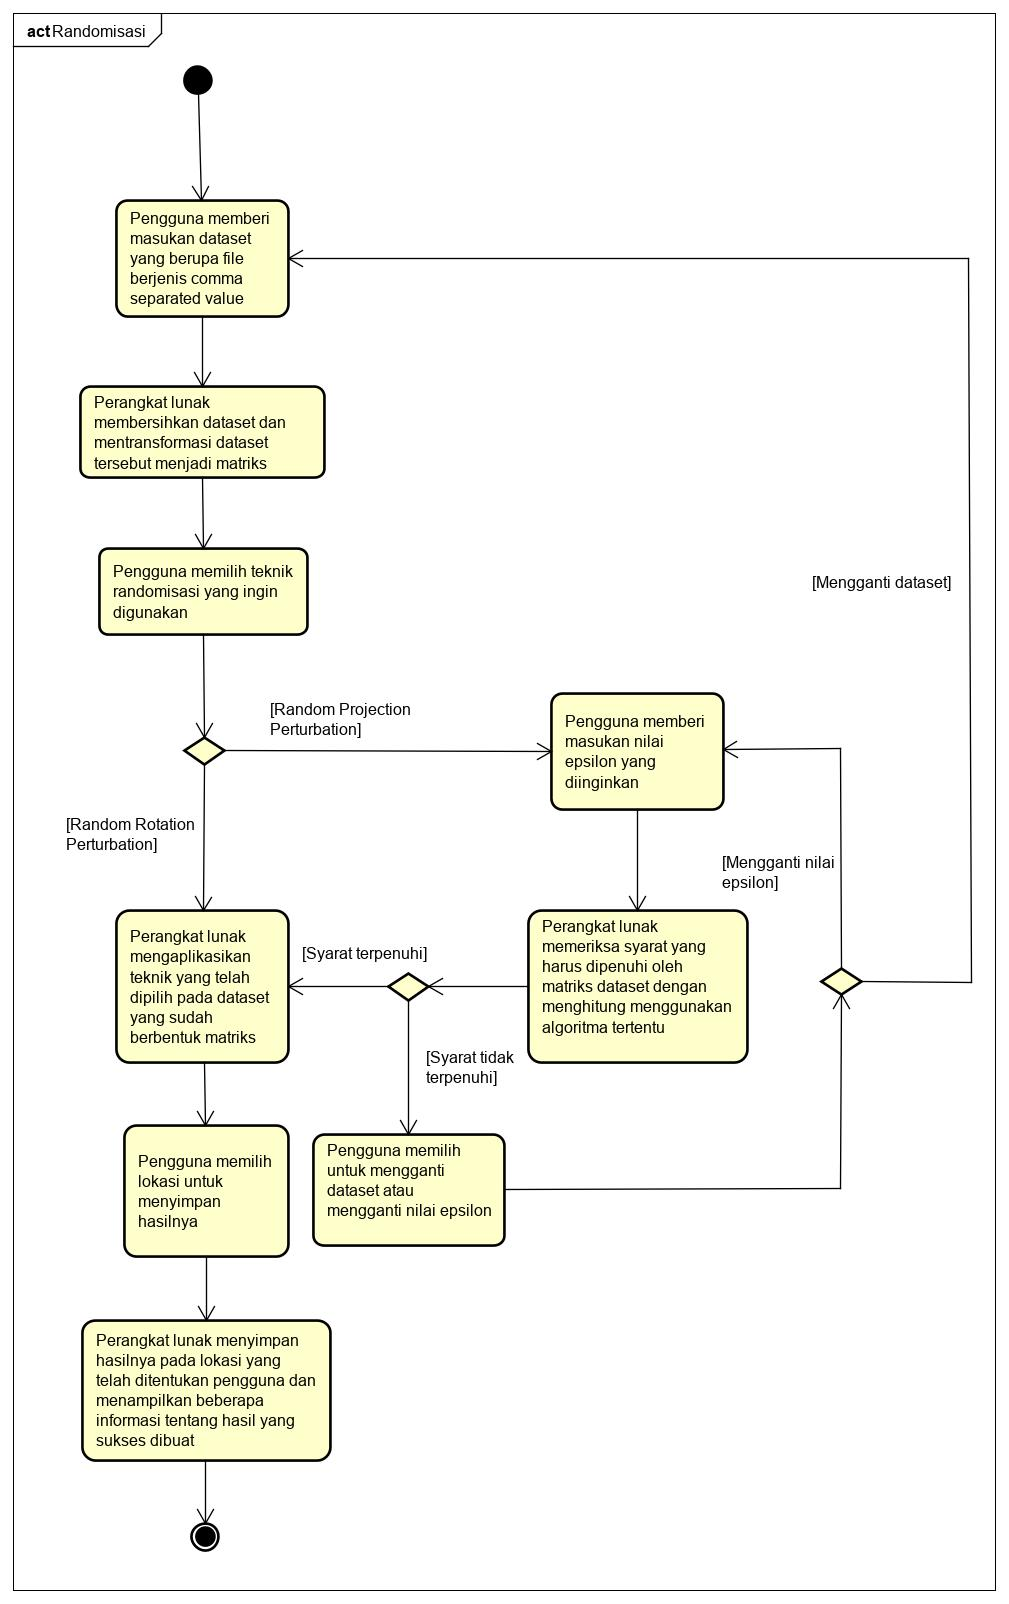
\includegraphics[scale=0.4]{activitydiagram}
			\caption{Diagram aktivitas perangkat lunak randomisasi}
			\label{fig:activitydiagram}
		\end{figure}

		\item \textbf{Melakukan analisis dan merancang diagram kelas perangkat lunak randomisasi}\\
		{\bf Status :} Ada sejak rencana kerja skripsi.\\
		{\bf Hasil :} Perancangan diagram kelas didasarkan pada analisis terhadap algoritma yang ingin diimplementasikan yaitu \textit{Random Rotation Perturbation} dan \textit{Random Projection Perturbation}, serta berdasarkan pada diagram aktivitas yang telah dibuat, dan dengan mempertimbangkan studi literatur, analisis masalah, dan studi kasus yang telah dilakukan pada kedua algoritma randomisasi yang ingin diimplementasikan. Detail dari diagram kelas perangkat lunak randomisasi pada Gambar~\ref{fig:classdiagram} adalah sebagai berikut.
		\begin{itemize}
			\item Kelas \textit{Perturbation} adalah kelas abstrak yang akan di-\textit{extend} oleh kelas yang mengimplementasikan algoritma \textit{Random Rotation Perturbation} dan \textit{Random Projection Perturbation}
			\item Kelas \textit{RandomRotationPerturbation} adalah kelas yang mengimplementasikan algoritma \textit{Random Rotation Perturbation}. Kelas ini merupakan \textit{subclass} dari kelas \textit{Perturbation}
			\item Kelas \textit{RandomProjectionPerturbation} adalah kelas yang mengimplementasikan algoritma \textit{Random Projection Perturbation}. Kelas ini merupakan \textit{subclass} dari kelas \textit{Perturbation}
			\item Kelas \textit{Matrix} adalah kelas untuk merepresentasikan matriks dan menyimpan nilai-nilai pada setiap elemen matriks. Kelas ini juga memiliki fungsi perkalian yang akan digunakan untuk implementasi algoritma \textit{Random Rotation Perturbation} dan \textit{Random Projection Perturbation}
			\item Kelas \textit{RandomTranslationMatrix} adalah kelas untuk membuat matriks translasi acak. Kelas ini adalah \textit{subclass} dari kelas \textit{Matrix}
			\item Kelas \textit{RandomRotationMatrix} adalah kelas untuk membuat matriks rotasi acak. Kelas ini adalah \textit{subclass} dari kelas \textit{Matrix}
			\item Kelas \textit{RandomProjectionMatrix} adalah kelas untuk membuat matriks proyeksi acak. Kelas ini adalah \textit{subclass} dari kelas \textit{Matrix}
			\item Kelas \textit{CSVPreprocessor} adalah kelas untuk menangani masukan \textit{dataset} berupa dokumen CSV yang akan direpresentasikan menjadi matriks. Kelas ini berguna untuk mengkonversi dokumen CSV menjadi matriks dan sebaliknya.
		\end{itemize}
		
		\begin{figure}
			\centering
			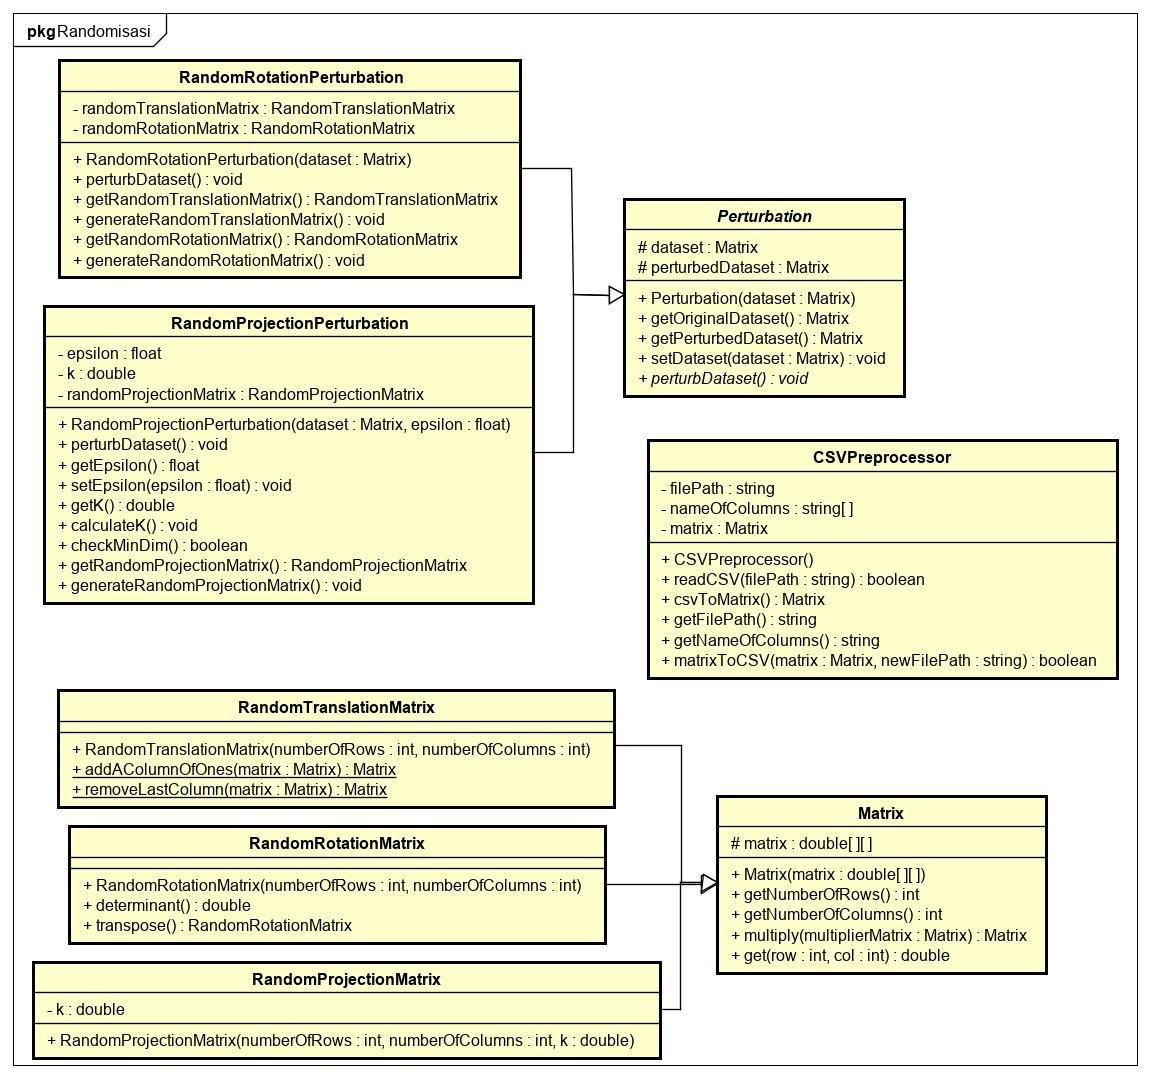
\includegraphics[scale=0.4]{classdiagram}
			\caption{Diagram kelas perangkat lunak randomisasi}
			\label{fig:classdiagram}
		\end{figure}

		\item \textbf{Menulis dokumen skripsi}\\
		{\bf Status :} Ada sejak rencana kerja skripsi.\\
		{\bf Hasil :} Penulisan dokumen skripsi telah dilakukan sampai hasilnya sekarang sudah ada bab 1 yang berisi pendahuluan, bab 2 yang berisi dasar teori, dan bab 3 yang berisi analisis masalah. Tetapi masih belum 100\% selesai, perlu adanya proses finalisasi.
		
	\end{enumerate}

\section{Pencapaian Rencana Kerja}
Langkah-langkah kerja yang berhasil diselesaikan dalam Skripsi 1 ini adalah sebagai berikut:
\begin{enumerate}
	\item Mempelajari dasar-dasar privasi data
	\item Mempelajari teknik \textit{Random Rotation Perturbation} dan \textit{Random Projection Perturbation} untuk \textit{privacy preserving data mining}
	\item Mempelajari teknik penambangan data yang akan digunakan
	\item Melakukan analisis terhadap teknik \textit{Random Rotation Perturbation} dan \textit{Random Projection Perturbation} serta bagaimana penerapannya dengan teknik penambangan data yang akan digunakan
	\item Menulis dokumen skripsi bab 1, 2, dan 3
\end{enumerate}



\section{Kendala yang Dihadapi}
%TULISKAN BAGIAN INI JIKA DOKUMEN ANDA TIPE A ATAU C
Kendala - kendala yang dihadapi selama mengerjakan skripsi :
\begin{itemize}
	\item Kesibukan lain yang menghabiskan banyak waktu seperti kuliah, kerja praktek, tugas-tugas mata kuliah lain, masalah pribadi dan hal-hal lainnya
	\item Kesulitan dalam melakukan studi literatur dengan membaca paper yang berbahasa Inggris dan penuh dengan rumus matematika
	\item Kesulitan dalam memahami konsep matematika yang ada pada teknik-teknik yang digunakan
	\item Kesulitan dalam mengetahui apa saja yang perlu ada di dokumen skripsi dan apa saja analisis yang harus dilakukan
	\item Kesulitan dalam menjaga mental untuk tetap semangat mengerjakan skripsi di kala masa-masa sulit
\end{itemize}

\vspace{1cm}
\centering Bandung, \tanggal\\
\vspace{2cm} \nama \\ 
\vspace{1cm}

Menyetujui, \\
\ifdefstring{\jumpemb}{2}{
\vspace{1.5cm}
\begin{centering} Menyetujui,\\ \end{centering} \vspace{0.75cm}
\begin{minipage}[b]{0.45\linewidth}
% \centering Bandung, \makebox[0.5cm]{\hrulefill}/\makebox[0.5cm]{\hrulefill}/2013 \\
\vspace{2cm} Nama: \pembA \\ Pembimbing Utama
\end{minipage} \hspace{0.5cm}
\begin{minipage}[b]{0.45\linewidth}
% \centering Bandung, \makebox[0.5cm]{\hrulefill}/\makebox[0.5cm]{\hrulefill}/2013\\
\vspace{2cm} Nama: \pembB \\ Pembimbing Pendamping
\end{minipage}
\vspace{0.5cm}
}{
% \centering Bandung, \makebox[0.5cm]{\hrulefill}/\makebox[0.5cm]{\hrulefill}/2013\\
\vspace{2cm} Nama: \pembA \\ Pembimbing Tunggal
}
\end{document}

